\documentclass{article}
\usepackage{graphicx}
\usepackage{hyperref}
\usepackage{amsmath}
\usepackage{times}
\usepackage{enumerate}

\textwidth=6.2in
\textheight=8.5in
%\parskip=.3cm
\oddsidemargin=.1in
\evensidemargin=.1in
\headheight=-.3in


%------------------------------------------------------------
% newcommand
%------------------------------------------------------------
\newcommand{\scscst}{\scriptscriptstyle}
\newcommand{\scst}{\scriptstyle}
\newcommand{\Robject}[1]{{\texttt{#1}}}
\newcommand{\Rfunction}[1]{{\texttt{#1}}}
\newcommand{\Rclass}[1]{\textit{#1}}
\newcommand{\Rpackage}[1]{\textit{#1}}
\newcommand{\Rexpression}[1]{\texttt{#1}}
\newcommand{\Rmethod}[1]{{\texttt{#1}}}
\newcommand{\Rfunarg}[1]{{\texttt{#1}}}

\usepackage{Sweave}
\begin{document}
\Sconcordance{concordance:GilbertWatson_LinearRegressionAssignment8.tex:GilbertWatson_LinearRegressionAssignment8.Rnw:%
1 28 1 1 0 71 1 1 2 17 0 1 2 1 1}


%------------------------------------------------------------
\title{Assignment 8}
%------------------------------------------------------------
\author{Gilbert Watson}
\date{Friday, December 6th, 2013}





\maketitle
\tableofcontents

%-------------------------------------------
\section{10.6}
%--------------------------------------------

Refer to Grocery retailer Problem 6.9:

\begin{enumerate}[a)]
\item{} Fit regression model (6.1) to the data using $X_1$ and $X_2$ only.
\item{} Prepare an added-variable plot for each of the predictor variables $X_1$ and $X_2$.
\item{} Do your plots in part(a) suggest that the regression relationships in the fitted regressior function in part(a) are inapprppriate for any of the predictor variables? Explain.
\item{} Obtain the fitted regression function in part(a) by separately regressing both $Y$ and $X_2$ or $X_1$, and then regressing the residuals in an appropriate fashion.
\end{enumerate}

\subsection{Answer:}

\begin{enumerate}[a)]

\item{} First, let's read in the data and estimate a simple model:
\begin{Schunk}
\begin{Sinput}
> library(xtable)
> grocery <- read.table(file="10.6.txt")
> names(grocery) <- c("labor.hours","cases","pct.labor","holiday")
> grocery.fit <- lm(labor.hours~cases+pct.labor,data=grocery)
> grocery.fitsum <- summary(grocery.fit)
> print(xtable(grocery.fitsum))
\end{Sinput}
% latex table generated in R 3.0.1 by xtable 1.7-1 package
% Fri Dec  6 01:26:10 2013
\begin{table}[ht]
\centering
\begin{tabular}{rrrrr}
  \hline
 & Estimate & Std. Error & t value & Pr($>$$|$t$|$) \\ 
  \hline
(Intercept) & 3995.4787 & 337.7660 & 11.83 & 0.0000 \\ 
  cases & 0.0009 & 0.0006 & 1.46 & 0.1517 \\ 
  pct.labor & 12.1205 & 39.7656 & 0.30 & 0.7618 \\ 
   \hline
\end{tabular}
\end{table}\end{Schunk}

\item{} To make added variable plots we must first estimate several models:
\begin{Schunk}
\begin{Sinput}
> yonx1 <- lm(labor.hours~cases,data=grocery)
> yonx2 <- lm(labor.hours~pct.labor,data=grocery)
> x1onx2 <- lm(pct.labor~cases,data=grocery)
> x2onx1 <- lm(cases~pct.labor,data=grocery)
\end{Sinput}
\end{Schunk}

Now we can plot residuals against each other:
\begin{Schunk}
\begin{Sinput}
> library(ggplot2)
> a <- qplot(x=x2onx1$residuals,
+       y=yonx2$residuals,
+       xlab="e(X1|X2)",
+       ylab="e(Y|X2)")
> a + geom_abline(intercept=0,slope=grocery.fit$coefficients[2])
\end{Sinput}
\end{Schunk}
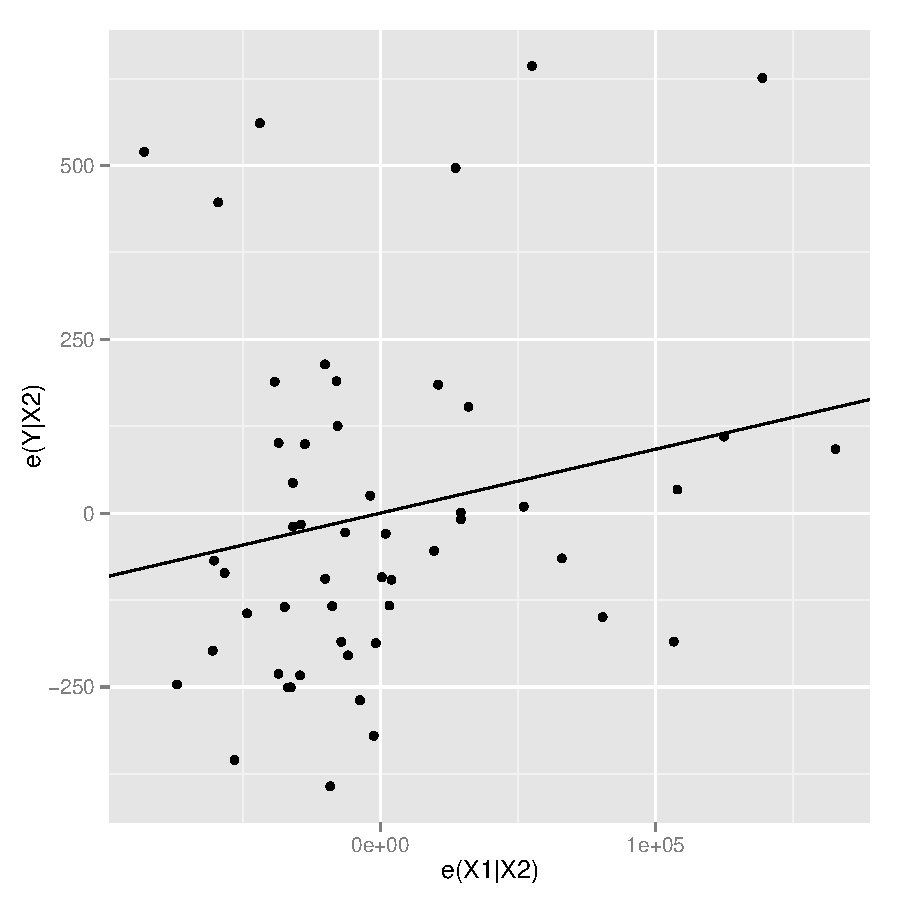
\includegraphics{Fig-addvarplots2}

\begin{Schunk}
\begin{Sinput}
> b <- qplot(x=x1onx2$residuals,
+       y=yonx1$residuals,
+       xlab="e(X2|X1)",
+       ylab="e(Y|X1)")
> b + geom_abline(intercept=0,slope=grocery.fit$coefficients[3])
\end{Sinput}
\end{Schunk}
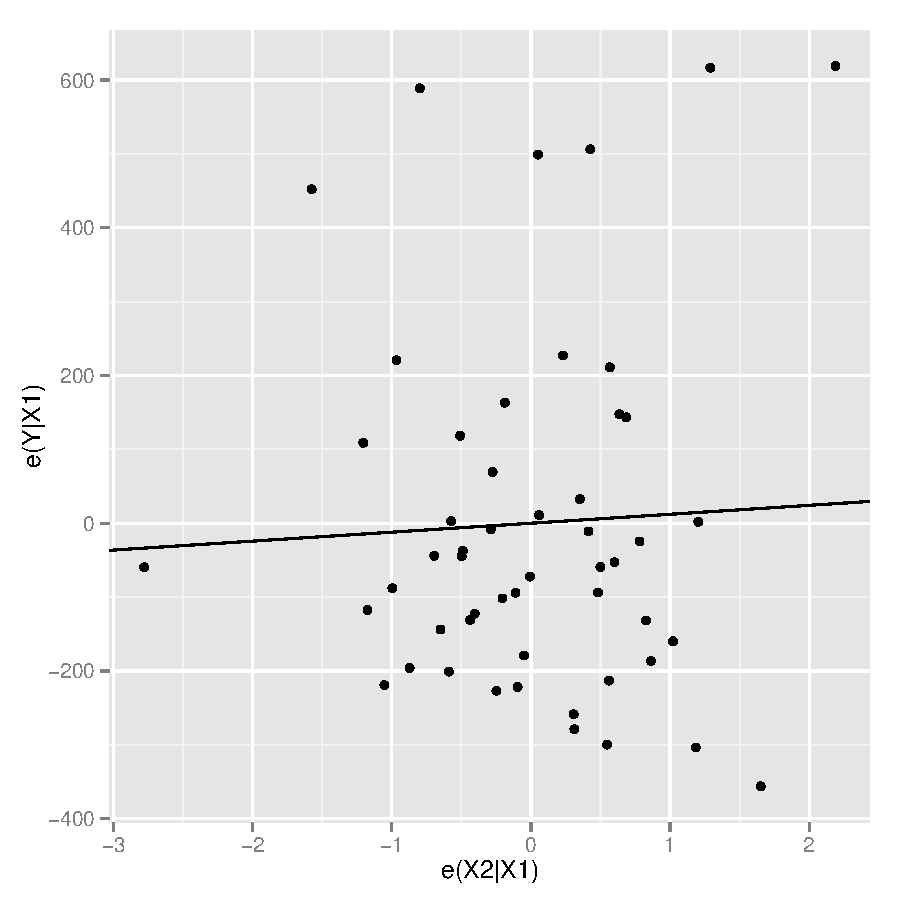
\includegraphics{Fig-addvarplots3}


\item{} 

The added variable plots suggest that the model is not aided by the addition of $X_2$. While the slope of the line in the first plot is quite different than a horizontal line, indicating that $X_1$ should probably be added to a model already containing $X_2$, the line for the second is almost horizontal, indicating that $X_2$ should not be added to a model already containing $X_1$.

\item{} 

First we must regress the residuals from above through the origin:
\begin{Schunk}
\begin{Sinput}
> originreg <- lm(yonx2$residuals~x2onx1$residuals-1)
> originreg$coefficients
\end{Sinput}
\begin{Soutput}
x2onx1$residuals 
    0.0009191639 
\end{Soutput}
\end{Schunk}
 
$$\epsilon{}\hat{(Y|X_2)} = 0.000919163915830026[\epsilon{}(X_1|X_2)]$$
$$[\hat{Y} - (4237.4687511802 + 17.036618933466X_2)] = 0.000919163915830026[X_1 - (263271.957683668 + 5348.44939715936X_2)]$$
$$\hat{Y} = 3995.47866762744 + 0.000919163915830026X_1 + 3995.47866762744X_2$$

\end{enumerate}

%-------------------------------------------
\section{10.12}
%--------------------------------------------

Refer to Commercial Properties Problem 6.18:

\begin{enumerate}[a)]
\item{} Obtain the studentized deleted residuals and identify any outlying $Y$ observations. Use the Bonferroni outlier test procedure with $\alpha{} = 0.1$. State the decision rule and conclusion.
\item{} Obtain the diagonal elements of the hat matrix. Identify any outlying $X$ observations.
\item{} The researcher wishes to estimate the rental rates of a property whose age is 10 years, whose operating expenses and taxes are 12.00, whose ocupancy rate is 0.05, and whose square footage is 350,000. Use (10.29) to determine whether this estimate will involve a hidden extrapolation.
\item{} Cases 61, 8, 3, and 53 appear to be outlying $X$ observations, and cases 6 and 62 appear to be outlying $Y$ observations. Obtain the DFFITS, DFBETAS, and Cook's distance values for each case to assess its influence. What do you conclude?
\end{enumerate}

\subsection{Answer:}

\begin{enumerate}[a)]

\item{} First let's read in the data and estimate a model:
\begin{Schunk}
\begin{Sinput}
> commProps <- read.table(file="10.12.txt")
> names(commProps) <- c("rental.rates","age","expenses","vacancy","sqft")
> commProps.fit <- lm(rental.rates~age+expenses+vacancy+sqft,data=commProps)
\end{Sinput}
\end{Schunk}

Now let's compute the studentized delted residuals and identify potential outliers
\begin{Schunk}
\begin{Sinput}
> library(MASS)
> stud.del.res <- studres(commProps.fit)
> qplot(seq(1,length(stud.del.res),1),abs(stud.del.res),
+       xlab="observation",
+       ylab="studentized delted residual")
\end{Sinput}
\end{Schunk}
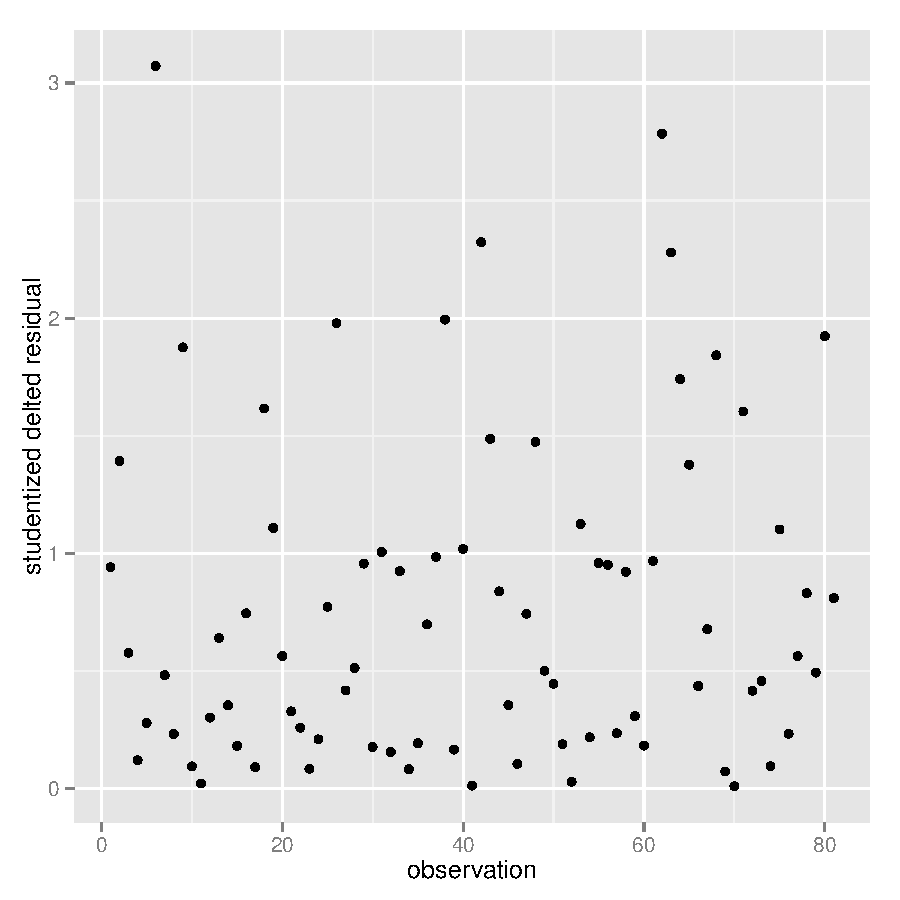
\includegraphics{Fig-massstuff}

Now let's calculate the Bonferroni critical value for outliers:
\begin{Schunk}
\begin{Sinput}
> alpha <- 0.1
> critical.t <- qt(1-alpha/(2*length(stud.del.res)),
+                  length(stud.del.res)-
+                    length(commProps.fit$coefficients))
> paste0("The critical value is t = ",critical.t)
\end{Sinput}
\begin{Soutput}
[1] "The critical value is t = 3.35660231603714"
\end{Soutput}
\begin{Sinput}
> paste0("Any studentized residuals > ",critical.t," ?  ",
+        any(abs(stud.del.res) > critical.t))
\end{Sinput}
\begin{Soutput}
[1] "Any studentized residuals > 3.35660231603714 ?  FALSE"
\end{Soutput}
\end{Schunk}

There are no outliers in the data by the bonferroni test. There aren't. I know what the next part of the question says and there aren't

\item{} Let's find the diagonals of the hat matrix, use it to find outliers, and print the observation number:
\begin{Schunk}
\begin{Sinput}
> diagonal <- lm.influence(commProps.fit)$hat
> threshold <- 2*(length(commProps.fit$coefficients)-1)/length(commProps$age)
> outliers <- as.vector(which(diagonal > threshold))
> paste(c("The outlier observations are:",outliers),collapse=" ")
\end{Sinput}
\begin{Soutput}
[1] "The outlier observations are: 3 8 9 43 53 54 61 65 80"
\end{Soutput}
\end{Schunk}

\item{} First let's compute $X_{new}$:
\begin{Schunk}
\begin{Sinput}
> xnew <- c(10,12.00,0.05,350000)
> xold <- as.matrix(commProps.fit$model[,setdiff(names(commProps.fit$model),
+                                      c("rental.rates"))])
\end{Sinput}
\end{Schunk}

Then let's find $h_{new,new}$ and see if it is greater than the threshold value:
\begin{Schunk}
\begin{Sinput}
> hnewnew <- t(xnew)%*%solve(crossprod(xold))%*%xnew
> hnewnew
\end{Sinput}
\begin{Soutput}
           [,1]
[1,] 0.05203178
\end{Soutput}
\end{Schunk}

$h_{new,new}$ is well within the range of the other diagonal entires of $\bf{H}$. It's prediction would not involve hidden extrapolation.

\item{} Let's find DFFITS, DFBETAS, and Cook's D for the following observations and make a table:
\begin{Schunk}
\begin{Sinput}
> library(xtable)
> weirdos <- c(61,8,3,53,6,62)
> diagnostics <- data.frame(DFFITS=dffits(commProps.fit)[weirdos],
+                           DFBETAS=dfbetas(commProps.fit)[weirdos],
+                           Cooks.D=cooks.distance(commProps.fit)[weirdos])
> diagnostics$`DFFITS > 1` <- abs(diagnostics$DFFITS) > 1
> diagnostics$`DFBETAS > 1` <- abs(diagnostics$DFBETAS) > 1
> diagnostics$`F Percentile` <- pf(diagnostics$Cooks.D,
+                                  4,
+                                  length(commProps$age)-4)
> print(xtable(diagnostics))
\end{Sinput}
% latex table generated in R 3.0.1 by xtable 1.7-1 package
% Fri Dec  6 01:26:11 2013
\begin{table}[ht]
\centering
\begin{tabular}{rrrrllr}
  \hline
 & DFFITS & DFBETAS & Cooks.D & DFFITS $>$ 1 & DFBETAS $>$ 1 & F Percentile \\ 
  \hline
61 & 0.64 & -0.06 & 0.08 & FALSE & FALSE & 0.01 \\ 
  8 & 0.12 & -0.01 & 0.00 & FALSE & FALSE & 0.00 \\ 
  3 & -0.28 & -0.23 & 0.02 & FALSE & FALSE & 0.00 \\ 
  53 & 0.53 & -0.02 & 0.05 & FALSE & FALSE & 0.01 \\ 
  6 & -0.87 & 0.20 & 0.14 & FALSE & FALSE & 0.03 \\ 
  62 & 0.69 & 0.28 & 0.09 & FALSE & FALSE & 0.01 \\ 
   \hline
\end{tabular}
\end{table}\end{Schunk}

From our table it is clear that none of the appearant outliers are influential. DFFITS and DFBETAS are all less than 1 for these values, and Cook's D for these values is in a very low percential of the associated F distribution.

\end{enumerate}

%-------------------------------------------
\section{10.20}
%--------------------------------------------

Refer to Lung pressure Problems 9.13 and 9.14. The subset regression model containing first-order terms for $X_1$ and $X_2$ and the cross-product term $X_1X_2$ is to be evaluated in detail.

\begin{enumerate}[a)]
\item{} Obtain the variance inflation factors. Are there any indications that serious multicollinearity problems are present? Explain.
\item{} Obtain the studentized deleted residuals and identify any outlying $Y$ observations. Use the Bonferroni outlier test procedure with $\alpha{} = .05$. State the decision rule and conclusion.
\item{} Cases 3, 8, imd 15 are moderately far outlying with respect to their $X$ values, and case 7 is relatively far outlying with respect to its $Y$ value. Obtain DFFITS, DFBETAS, and Cook's distance values for these cases to assess their influence. What do you conclude?
\end{enumerate}

\subsection{Answer:}

\begin{enumerate}[a)]

\item{} Let's first read in the data and estimate the model:
\begin{Schunk}
\begin{Sinput}
> Lung <- read.table(file="10.20.txt")
> names(Lung) <- c("arterial.pressure","emptying.rate","ejection.rate","blood.gas")
> Lung.fit <- lm(arterial.pressure~emptying.rate*ejection.rate,
+                data=Lung)
\end{Sinput}
\end{Schunk}

Now let's obtain the variance inflation factors and $\bar{VIF}$:
\begin{Schunk}
\begin{Sinput}
> library(car)
> vif <- vif(Lung.fit)
> bar.vif <- mean(vif)
> vif
\end{Sinput}
\begin{Soutput}
              emptying.rate               ejection.rate 
                   5.431477                   11.639560 
emptying.rate:ejection.rate 
                  22.474469 
\end{Soutput}
\begin{Sinput}
> bar.vif
\end{Sinput}
\begin{Soutput}
[1] 13.18184
\end{Soutput}
\end{Schunk}

Yes, multicollinearity is an issue. All VIF values are above 1 and the interaction term's value is far above the mean VIF.

\item{} Are there any studentized deleted residuals greater than the critical value?
\begin{Schunk}
\begin{Sinput}
> stud.del.res <- studres(Lung.fit)
> alpha <- 0.05
> critical.t <- qt(1-alpha/(2*length(stud.del.res)),
+                  length(stud.del.res)-
+                    length(Lung.fit$coefficients))
> paste0("The critical value is t = ",critical.t)
\end{Sinput}
\begin{Soutput}
[1] "The critical value is t = 3.59890216225008"
\end{Soutput}
\begin{Sinput}
> paste0("Any studentized residuals > ",critical.t," ?  ",
+        any(abs(stud.del.res) > critical.t))
\end{Sinput}
\begin{Soutput}
[1] "Any studentized residuals > 3.59890216225008 ?  FALSE"
\end{Soutput}
\end{Schunk}

The decision rule is that if the studentized deleted residual is greater than the critical value, $3.59890216225008$, then we reject the null hypothesis that the outcome value is not an outlier. No studentized deleted residuals are greater than this critical value in this case, so we conclude that none of the $Y$ values are outliers.

\item{} Let's build a table to assess observation influence:
\begin{Schunk}
\begin{Sinput}
> weirdos <- c(3,8,15,7)
> diagnostics <- data.frame(DFFITS=dffits(Lung.fit)[weirdos],
+                           DFBETAS=dfbetas(Lung.fit)[weirdos],
+                           Cooks.D=cooks.distance(Lung.fit)[weirdos])
> diagnostics$`DFFITS > 1` <- abs(diagnostics$DFFITS) > 1
> diagnostics$`DFBETAS > 1` <- abs(diagnostics$DFBETAS) > 1
> diagnostics$`F Percentile` <- pf(diagnostics$Cooks.D,
+                                  3,
+                                  length(Lung$arterial.pressure)-3)
> print(xtable(diagnostics))
\end{Sinput}
% latex table generated in R 3.0.1 by xtable 1.7-1 package
% Fri Dec  6 01:26:11 2013
\begin{table}[ht]
\centering
\begin{tabular}{rrrrllr}
  \hline
 & DFFITS & DFBETAS & Cooks.D & DFFITS $>$ 1 & DFBETAS $>$ 1 & F Percentile \\ 
  \hline
3 & -0.68 & -0.65 & 0.12 & FALSE & FALSE & 0.05 \\ 
  8 & -4.78 & -1.55 & 4.99 & TRUE & TRUE & 0.99 \\ 
  15 & 0.17 & -0.02 & 0.01 & FALSE & FALSE & 0.00 \\ 
  7 & 1.75 & 1.45 & 0.46 & TRUE & TRUE & 0.29 \\ 
   \hline
\end{tabular}
\end{table}\end{Schunk}

We can conclude from this table that observations 8 and 7 are unduly influential to the model. They both have DFFITS and DFBETAS greater than 1 and Cook's D's that have a high percential ranking.

\end{enumerate}

%-------------------------------------------
\section{10.23}
%--------------------------------------------

Show that (10.37) is algebraically equivalent to (1O.33a).

\subsection{Answer:}

%-------------------------------------------
\section{System Information}
%--------------------------------------------

\begin{Schunk}
\begin{Sinput}
> sessionInfo();
\end{Sinput}
\begin{Soutput}
R version 3.0.1 (2013-05-16)
Platform: x86_64-apple-darwin10.8.0 (64-bit)

locale:
[1] en_US.UTF-8/en_US.UTF-8/en_US.UTF-8/C/en_US.UTF-8/en_US.UTF-8

attached base packages:
[1] stats     graphics  grDevices utils     datasets  methods   base     

other attached packages:
[1] car_2.0-19      MASS_7.3-26     ggplot2_0.9.3.1 xtable_1.7-1   

loaded via a namespace (and not attached):
 [1] colorspace_1.2-2   dichromat_2.0-0    digest_0.6.3       grid_3.0.1        
 [5] gtable_0.1.2       labeling_0.2       munsell_0.4.2      nnet_7.3-6        
 [9] plyr_1.8           proto_0.3-10       RColorBrewer_1.0-5 reshape2_1.2.2    
[13] scales_0.2.3       stringr_0.6.2      tools_3.0.1       
\end{Soutput}
\end{Schunk}

\end{document}
